\subsection{Aufbau}
Der Versuch besteht aus mehreren einzelnen Vorrichtungen. Hauptteile eben dieser sind:
\begin{itemize}
\item{Streuer}
\item{Geiger-Müllerzählrohr}
\item{Kupferröntgenröhre}
\end{itemize}
Im Falle des vorliegenden Versuches besteht der Streuer aus einem LiF-Kristall und einem Plexiglasquader. 
Die Messung und Einstellung verschiedener Winkel findet an einem Rechner statt. Es bietet sich an dem Programm des Rechners 
die Drehvorgänge zu überlassen, diese können aber auch manuell ausgeführt werden. 
Die wichtigen verstellbaren Parameter am Rechner sind:
\begin{itemize}
\item{Messart}
\item{Drehmodus}
\item{Kristallwinkel}
\item{Integrationszeit}
\end{itemize}
 
\begin{figure}
    \centering
    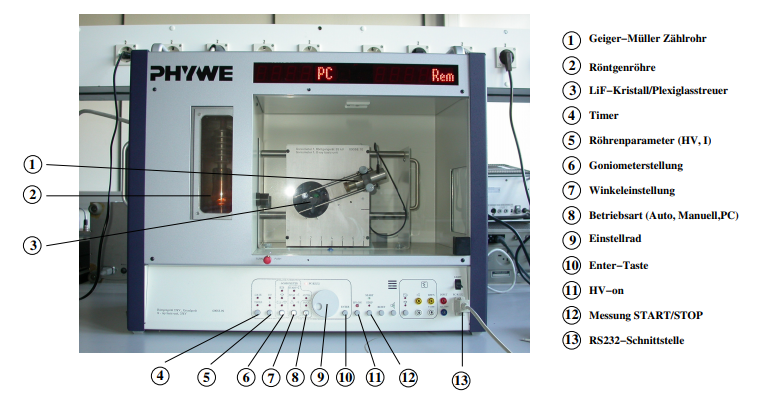
\includegraphics[width=\textwidth]{bilder/Screenshot 2021-01-29 104244.png}
    \caption{Rechner, Messgerät und Konfigurator \cite{skript}. } 
    \label{fig:Rechner}
\end{figure}

\subsection{Durchführung}
Über das ganze Experiment bleiben zwei Werte konstant, die zu Beginn eingestellt werden müssen.
Diese Werte werden als Beschleunigungsspannung zusammen mit einem Emissionsstrom gewählt. 
\begin{align*}
\text{Beschleunigungsspannung} &  \hspace{1 cm} 35 \hspace{0.1 cm}\si{kv} \\
\text{Emissionsstrom} &  \hspace{1 cm}   1 \hspace{0.1 cm} \si{mA}\\
\end{align*}
Das Emissionsspektrum wird mit einer 2mm Blende und dem LiF-Kristall gemessen. 
Dazu wird vorab das Röntgenspektrum herausgefunden. Mit den folgenden Einstellungen lassen sich die gesuchten Werte finden:
\begin{itemize}
\item{Winkelzuwachs $\Delta \theta = 0.2 \textdegree$}
\item{Integrationszeit $\Delta t = 5 \si{s} \text{bis} 10 \si{s}$}
\end{itemize}
Nach Abnahme der Werte wird zur Bestimmung der Compton-Wellenlänge ein Aluminiumabsorber vor die 2 mm Blender gestellt.
Es Folgen Messungen von $\text{N}_{AL}(\theta)$ und $\text{N}_{0}(\theta)$, also einmal mit Absorber und das andere mal ohne.
\\
\newline
Der nächste Wechsel ist von der 2 mm auf die 5 mm Blende. Parallel dazu wird der LiF-Kristall durch den Plexiglasstreuer getauscht
Die nächsten Messungen erfolgen manuell mit folgenden Parametern
\begin{itemize}
\item{$\theta_{\text{Kristall}}  = 45 \textdegree$}
\item{$\theta_{\text{Geiger-Müller-Zählrohr}}  = 45 \textdegree$}
\end{itemize}
Ziel der Messung ist die Intensität $I_0$ der Kupfer Röhre.
Hierbei wird darauf geachtet jeweils zwei unabhängige Versuchsdurchläufe zu gewährleisten mit einer Messzeit von $t > \SI{300}{\second}$.
Das führt zu einer genaueren Bestimmung der Werte unter Kleinhaltung des Fehlers.
Die Transmission $T_1$ wird mit Hilfe des Aluminiumabsorbers gemessen. Dieser wird dafür zwischen Röntgenröhre und Streukörper in den Strahlengang
gebracht. Analog dazu erfolgt die Messung der Transmission $T_2$. Hier wird lediglich der Absorber zwischen Streukörper und Geiger-Müllerzählrohr gelegt. (Anstelle der vorherigen Konfiguration)